\documentclass{article}

% if you need to pass options to natbib, use, e.g.:
\PassOptionsToPackage{numbers, compress}{natbib}
% before loading neurips_2026

% The authors should use one of these tracks.
% Before accepting by the NeurIPS conference, select one of the options below.
% 0. "default" for submission
\usepackage{tabularx}
\usepackage{xcolor}
% the "default" option is equal to the "main" option, which is used for the Main Track with double-blind reviewing.
\usepackage{fvextra} % for Unicode in verbatim
% 1. "main" option is used for the Main Track
%  \usepackage[main]{neurips_2026}
% 2. "position" option is used for the Position Paper Track
%  \usepackage[position]{neurips_2026}
% 3. "eandd" option is used for the Evaluations & Datasets Track
 % \usepackage[eandd]{neurips_2026}
% 4. "creativeai" option is used for the Creative AI Track
%  \usepackage[creativeai]{neurips_2026}
% 5. "sglblindworkshop" option is used for the Workshop with single-blind reviewing
 % \usepackage[sglblindworkshop]{neurips_2026}
% 6. "dblblindworkshop" option is used for the Workshop with double-blind reviewing
  \usepackage[dblblindworkshop]{neurips_2026}
% 7. "education" option is used for the Education Track
%  \usepackage[education]{neurips_2026}


% After being accepted, the authors should add "final" behind the track to compile a camera-ready version.
% 1. Main Track
 % \usepackage[main, final]{neurips_2026}
% 2. Position Paper Track
%  \usepackage[position, final]{neurips_2026}
% 3. Evaluations & Datasets Track
 % \usepackage[eandd, final]{neurips_2026}
% 4. Creative AI Track
%  \usepackage[creativeai, final]{neurips_2026}
% 5. Workshop with single-blind reviewing
%  \usepackage[sglblindworkshop, final]{neurips_2026}
% 6. Workshop with double-blind reviewing
%  \usepackage[dblblindworkshop, final]{neurips_2026}
% Note. For the workshop paper template, both \title{} and \workshoptitle{} are required, with the former indicating the paper title shown in the title and the latter indicating the workshop title displayed in the footnote.
% For workshops (5., 6.), the authors should add the name of the workshop, "\workshoptitle" command is used to set the workshop title.
\workshoptitle{NeurIPS 2026 Workshop on World Models in Physical AI}
% 7. Education Track
% \usepackage[education, final]{neurips_2026}

% "preprint" option is used for arXiv or other preprint submissions
 % \usepackage[preprint]{neurips_2026}

% to avoid loading the natbib package, add option nonatbib:
%    \usepackage[nonatbib]{neurips_2026}

\usepackage[utf8]{inputenc} % allow utf-8 input
\usepackage[T1]{fontenc}    % use 8-bit T1 fonts
\usepackage{hyperref}       % hyperlinks
\usepackage{url}            % simple URL typesetting
\usepackage{booktabs}       % professional-quality tables
\usepackage{amsfonts}       % blackboard math symbols
\usepackage{nicefrac}       % compact symbols for 1/2, etc.
\usepackage{microtype}      % microtypography
\usepackage{xcolor}         % colors

\usepackage{amsmath}

\usepackage{todonotes}
\setuptodonotes{size=\tiny}


% Note. For the workshop paper template, both \title{} and \workshoptitle{} are required, with the former indicating the paper title shown in the title and the latter indicating the workshop title displayed in the footnote. 
\title{Mechanical Validity Does Not Imply World-Model Fidelity: Evaluating LLM-Generated Executable POSGs}


% The \author macro works with any number of authors. There are two commands
% used to separate the names and addresses of multiple authors: \And and \AND.
%
% Using \And between authors leaves it to LaTeX to determine where to break the
% lines. Using \AND forces a line break at that point. So, if LaTeX puts 3 of 4
% authors names on the first line, and the last on the second line, try using
% \AND instead of \And before the third author name.


\author{Anonymous Authors}


\begin{document}


\maketitle


\begin{abstract}
  %The abstract paragraph should be indented \nicefrac{1}{2}~inch (3~picas) on both the left- and right-hand margins. Use 10~point type, with a vertical spacing (leading) of 11~points. The word \textbf{Abstract} must be centered, bold, and in point size 12. Two line spaces precede the abstract. The abstract must be limited to one paragraph.
World models used for planning must capture action-conditioned dynamics, not merely satisfy an executable interface. We study whether large language models can translate natural-language situations into executable partially observable stochastic games (POSGs). Our 44-scenario benchmark has three empirical tracks with different evidence regimes. The game track evaluates five models on nine reference-backed games over three runs (135 first-pass trials); the situational track provides a balanced completed subset of 135 first-pass trials on S1--S9; and the cultural track evaluates 84 JSON candidates from three models under anonymized and country-named prompts. First-pass mechanical/Lane-1 validity is respectively 124/135, 107/135, and 75/84. In the game track, the 134 artifacts passing a post-hoc Lane-1 audit obtain mean fallback structural F1 0.7178, with only 32 exact fallback matches. Cultural location disclosure changes mean automated semantic scores by at most 0.007 in the three observed model pairs, but these diagnostics are not human validated. Across tracks, mechanical validity varies with scenario regime and does not establish structural or semantic fidelity.
\end{abstract}

\section{Introduction}
\label{sec:intro}
\paragraph{Motivation and Core Challenge}
% \todo{i'm not sure "formatting" is the right phrase. also, i'm not sure "safe-by-design" is essential. what if we use the title "Can LLMs Construct Formal, Situational World Models for AI Agents? Test Cases, Evaluation Methods, and First Results"}
% \todo{make sure all official general neurips and workshop-specific formatting rules are followed!}
% \todo{we must agree on an author list and ordering since that is probably part of the online submission form. i suggest alphabetical ordering for simplicity, unless someone vetos this.}
Many approaches to ``safe-by-design'' AI systems \citep{dalrymple2024guaranteedsafeaiframework} rely on formal, tractable world models to evaluate safety-critical metrics such as action reversibility \citep{eysenbach2018leave}, state reachability \citep{krakovna2020avoiding}, agent empowerment \citep{klyubin2005empowerment}, or the effects on capabilities and resulting (dis)empowerment of the humans an agent interacts with \citep{salge2017empowerment,heitzigfair}. 
Traditional world models such as neural network approximations or large Bayesian networks \citep{amodei2016concrete,ha2018world} often lack structural transparency and/or symbolic grounding required for formal verification  \citep{konidaris2018from}, or are too large for tractable planning. 

Generating formal, ``situational world models'' that are suitable for a given situation and a given level of granularity of the decision making process just in time is a possible way to address transparency and tractability.
A significant challenge for such an approach is that the suitability criteria for a situational world model depend on the specific context. In industrial, single-agent planning scenarios with predominantly deterministic dynamics, suitability mostly means correctness and is relatively easy to assess: the model either accurately represents the environment's mechanics at the given level of detail, or it does not, and its predictions can often be verified against the actual dynamics.

In complex real-world situations with several individuals, such clarity often fades. There is not just one accurate model---various plausible models emphasize different stakeholders, choices, and outcomes. It becomes easy to overlook an ethically significant aspect: a party involved may not take explicit action, an option might only be significant under uncertain cultural norms, and a consequence, while unlikely, may be severe. In this situation, assessing the balance between tractability and sufficient detail is challenging. If the model is too simple, it might miss the key distinction on which the safe action depends, and there is no ground-truth reference available against which to detect the loss.

Addressing this trade-off might require a hierarchical approach, where situations are described at multiple levels of granularity and refined only on demand. %where safety-relevant distinctions demand it. 
In this paper, we focus on a single layer of such a hierarchy: generating and evaluating one situational world model per scenario.
% \todo{i like this very much so far!}

\paragraph{LLMs as World Model Generators}
This work investigates whether modern Large Language Models (LLMs) can bridge the gap between unstructured, real-world scenario descriptions and formal safety environments by constructing Partially Observable Stochastic Games (POSGs)encoded in a structured format (JSON or Python). For single-agent, largely deterministic settings, literature shows that LLMs are able to produce correct models expressed in planning languages such as PDDL, and to generate executable ``code world models'' for model-based planning \citet{cao2025large,dainese2024generating}. For complex situations with multiple affected humans, this capability has been studied far less, and arguably PDDL or its extensions might not (yet) be the right data structures to represent them.

The multi-human setting also faces failure modes that are specific to LLM generation and largely absent from the deterministic single-agent case:
\begin{itemize}
    \item \textbf{Invention of details:} the model introduces facts, quantities, or intentions that are absent from the situation description, such as an invented feature, a freely made-up probability, an attributed goal, or a fabricated participant. If the formal schema (e.g. a fully instead of partially observed stochastic game, or the requirement to specify ``rewards'') requires commitment to quantities the text underdetermines, this failure is invited rather than incidental.
    \item \textbf{Omission of inferable structure:} the model overlooks a stakeholder, state variable, or behavioral option that is not explicitly mentioned but that general world understanding would recognize as plausibly present and safety-relevant. For example, a custodial party who never acts explicitly but whose interests determine the safe outcome.
    \item \textbf{Bias, especially under cultural uncertainty:} when the situation leaves the cultural context underspecified, the model may resolve it according to a dominant prior, systematically privileging particular interpretations. On the other hand, when a cultural context is specified, the model might take up clich\'ees and preconceptions from the LLM's training data.
\end{itemize}

These are not merely syntactic or mechanical quality failures. Each can occur in an otherwise well-formed world model while materially changing the conclusions of a downstream planner. This distinction motivates our evaluation framework: mechanical validity alone is insufficient, and evaluation must additionally test structural fidelity, semantic coverage, and unsupported invention.
% \todo{i don't understand why those issues are not quality issues? isn't unbiasedness not a quality?}

\paragraph{Key Contributions}
In this workshop paper, we contribute:
\begin{itemize}
    \item A curated corpus of 44 test-case situations spanning toy, game, situational, and cultural scenarios, tiered by how much ground truth is available.
    \item A generation pipeline that prompts LLMs to produce POSG world models in a structured JSON schema or as python classes implementing a given abstract base class.
    \item A multi-lane evaluation framework separating mechanical validity, reference-backed structural comparison, and diagnostic semantic coverage.
    \item Three complementary empirical tracks: reference-backed games, open-ended situational Python POSGs, and culturally contextualized JSON POSGs, with explicit evidence boundaries for each.
\end{itemize}


\section{Related Work}
\label{sec:related_work}

\paragraph{Safe-by-Design AI and Empowerment}
%Formal safety criteria require explicit modeling of state-action-state transitions to ensure non-irreversible actions and maintain bounded agent influence.
A line of work aims to keep AI systems safe by preserving human choices rather than telling AI agents what to do. Methods like attainable-utility preservation \citep{turner2020conservative} and reachability-based side-effect penalties \citep{krakovna2020avoiding} aim to make AI agents act cautiously, but quantify this from the agent's own perspective rather than measuring human capability. In contrast, empowerment-based goals aim to preserve or increase the human's capability to influence outcomes. Recent research formalises a fair, risk- and inequality-averse aggregate of human power as a formal AI objective \citet{heitzigfair}. All these methods rely on a clear state–action–state framework: computing reversibility, reachability, or power presupposes a world model that already contains the relevant stakeholders, options, and consequences. This is what makes the quality of a generated world model a safety concern rather than a modelling convenience, and what our evaluation is designed to check.

\paragraph{LLMs for Environment Synthesis and Code Generation}
%Prior research explores generating grid-worlds or domain-specific languages (DSLs) via LLMs, but lacks comprehensive multi-agent stochastic game modeling.
LLMs have been used to synthesize environments and domain-specific programs, including generating grid worlds, task specifications, and planning-language descriptions. \citet{dainese2024generating} generated code-world models (Python implementations of an environment's dynamics) for model-based reinforcement learning. They argue that calling code at planning time, rather than an LLM, yields greater precision, interpretability, and efficiency, and they validate the generated code against unit tests and environment trajectories. \citet{cao2025large} survey the broader LLM planning literature, categorizing methods into external-module-augmented, finetuning-based, and search-based approaches. This work focuses on single-agent settings and assumes access to a ground truth (an executable environment or a verifiable plan) against which generated artifacts can be evaluated. Our problem setting differs on both assumptions: we consider a multi-player (AIs and humans) stochastic game, and in realistic applications there is no unique ground-truth model to validate against, which motivates the evaluation design in Section~\ref{subsec:evaluation_framework}.

\paragraph{World-Model Evaluation}
%Discussion of existing benchmarking tools for state-space coverage, LLM-as-a-judge reliability, and structural graph analysis in synthetic environments.
Evaluating synthesised situational world models draws on several metrics, including mechanical validity checks (well-formedness, probability normalisation, reachability of generated states), structural and graph-based comparison of state-transition topologies, and LLM-as-a-judge protocols for qualities that are difficult to verify automatically. Existing metrics often assume the existence of a reference model, failing to address situations where correctness is genuinely indeterminate and must be evaluated against human-specified expectations rather than a ground-truth model. We combine mechanical, structural, and judgement-based metrics into a single framework in Section~\ref{subsec:evaluation_framework}.

\section{Benchmark and Evaluation Method}
\label{sec:method}

\subsection{Preliminaries}
\label{subsec:preliminaries}

\paragraph{Partially Observable Stochastic Games (POSG)}
A formal POSG is defined as a tuple $\mathcal{M} = \langle \mathcal{N}, \mathcal{S}, \mathcal{A}=\{\mathcal{A}_i\}_{i \in \mathcal{N}}, \mathcal{P}, \mathcal{O}=\{\mathcal{O}_i\}_{i \in \mathcal{N}}, \Omega \rangle$, where $\mathcal{N}$ is a set of players which may include humans and AI systems,
%\todo{let's use the established game-theoretical term `player' for humans+AIs, and reserve `agent' for AI systems?}
$\mathcal{S}$ is the set of (potentially hidden) states, $\mathcal{A}_i$ is the action space for player $i$, $\mathcal{P}(s' \mid s, a)$ defines state transition probabilities given joint action $a=\{a_i\}_{i\in\mathcal N}$, and $\Omega:\mathcal S\times\mathcal A\times\mathcal S\to\mathcal O$ is a (deterministic) observation function representing what every player will actually observe after a transition.

\paragraph{The Situation--World-Model--Planner Architecture}
We adopt a modular, neutral baseline architecture decoupling the world model from policy synthesis:
\begin{enumerate}
    \item \textbf{Perception / Prompt Input}: The natural-language scenario or situation description.
    \item \textbf{Situational World Model (LLM Output)}: A neutral, predictive resource representing valid state-space transitions without embedded agent biases.
    \item \textbf{Planner / Decision Engine}: The downstream decision algorithm executing policy searches over the synthesized world model (e.g. some form of dynamic programming or model-based reinforcement learning).
\end{enumerate}

\paragraph{Output Formats for Representing Situational World Models}
Models are formalized as POSGs encoded either as explicit JSON structures listing individual transitions, obeying a prescribed schema (for small state spaces), or as executable Python classes generating transitions programmatically, extending a prescribed Abstract Base Class (for more complex environments).
% \todo{I also like sections 2 and 3 very much so far! you're on a good track!!}

% \begin{figure}
%     \centering
%     \includegraphics[width=1\linewidth]{world model generation.png}
%     \caption{World-Model Generation.}
%     \label{fig:world}
% \end{figure}

\section{Dataset and Benchmark Suite}
\label{sec:dataset}

To evaluate world-model synthesis under realistic conditions, we construct a specialized benchmark suite that prioritizes structural diversity, domain coverage, and distinct multi-player trade-offs over brute-force data volume. Rather than inflating dataset size through trivial parameter variations—such as resizing grids or swapping entity labels—each scenario introduces a unique combination of partial observability, state-space topology, non-zero-sum payoff structure, and safety-critical choices.

The dataset is structured into four primary domain tiers, each designed to isolate specific reasoning challenges ranging from low-level transition dynamics to high-level normative constraints:
(1) toy environments with tightly specified mechanics; (2) simple games with known rules and reference structure; (3) situational scenarios involving asymmetric stakeholders, resources, or consequences; and (4) culturally contextualized scenarios in which relevant structure or norms may be underspecified.
% \todo{please confirm that this is a better description than ``Canonical POSGs and game-theoretic equilibria''}


%%%%%%%%%%% deactivated:
\iffalse
\begin{verbatim}
world-model-suite/data/
├── README.md
└── Test_Cases/
    ├── 01_toy/           # Mechanics & exact transition baselines
    ├── 02_situational/   # Resource conflicts & asymmetric stakes
    ├── 03_game/          # Canonical POSGs & game-theoretic equilibria
    └── 04_cultural/      # Social hierarchies & regional norm shifts
\end{verbatim}
\fi
%%%%%%%%%%%%

To provide a granular view of the dataset's scope, Table~\ref{tab:dataset_taxonomy} outlines the scenario distribution across all four categories, detailing the explicit case counts and representative state-action dimensions.

\begin{table*}[t]
\centering
\small
\caption{Taxonomy of the benchmark suite detailing scenario counts, state-space scale ($|S|$), and action-space dimensionality ($|A|$) across tiers.}
\label{tab:dataset_taxonomy}
\begin{tabularx}{\linewidth}{l X c c c}
\toprule
\textbf{Tier} & \textbf{Category} & \textbf{Count} & \textbf{State Space $|S|$} & \textbf{Action Space $|A|$} \\
\midrule
\textbf{01} & Toy Environments & 10 & $10^1 - 10^2$ & $2 - 4$ \\
\textbf{02} & Situational Dilemmas & 11 & $10^3 - 10^5$ & $4 - 10$ \\
\textbf{03} & Simple Games & 9 & $10^1 - 10^3$ & $2 - 6$ \\
\textbf{04} & Cultural Dynamics & 14 & Unbounded & $6 - 15$ \\
\midrule
\textbf{Total} & \textbf{Benchmark Suite} & \textbf{44} & -- & -- \\
\bottomrule
\end{tabularx}
\end{table*}
Table 1 characterizes the benchmark. %rather than model performance; validation and evaluation outcomes are reported separately in Section 5 to avoid conflating dataset composition with evaluation results.

Following that line of work, we develop a benchmark design that explicitly avoids overpopulating the suite with syntactically similar scenarios. By shifting focus toward qualitative variations rather than repetitive scaling, we aim to help establishing whether large language models can generalize across distinct behavioral landscapes rather than simply memorizing repetitive structural patterns.

We also highlight normative and contextual uncertainty across complex domain boundaries. Scenarios within the cultural tier present ambiguous social hierarchies where appropriate actions depend heavily on localized norms rather than universal safety constraints. These cases are designed to test whether generated world models introduce culturally specific assumptions that are unsupported by the scenario description, and whether those assumptions vary when contextual information is changed or withheld.

% \todo{if we indeed find that they do, that finding must go into sec 5, not here.}

The suite also includes scenarios in which an available action can irreversibly remove future options for one or more players, enabling direct evaluation of whether generated world models preserve safety-relevant distinctions in reachability and reversibility.

% \todo{Someone commented: Verify whether the final camera-ready layout requires breaking down the exact JSON schema validation pass rate per tier alongside Table~\ref{tab:dataset_taxonomy}.} % that was not my comment... (Jobst)

\subsection{World-Model Generation Pipeline}
% \todo{Jobst: good structure!}
\label{subsec:wm_generation}

%\paragraph{Natural-Language-to-POSG Code Synthesis}
We provide either the prescribed JSON schema or Python \texttt{AbstractPOSG} interface in the generation prompt and require the model to represent the players, decision-relevant states, available actions, transition dynamics, and player observations through that interface. Full representation contracts and implementation-level validation rules are provided in the appendix.

%\paragraph{Standardized Prompt Blueprint and Constrained Schemas}
Prompt variants impose progressively stronger, task-independent representation constraints, including interface compliance, valid transition distributions, consistency between states and actions, and preservation of the decision horizon described by the scenario. Importantly, generated models are evaluated as produced: unsupported invention, omission of relevant structure, and semantic inconsistencies are treated as evaluation outcomes rather than silently repaired during post-processing.

%%%%%%%%% deactivated because redundant with previous text:
\iffalse
\paragraph{Handling Complex Scenarios and Dilemmas}
Extending world-model generation beyond simple toy games to multi-agent situational dilemmas (e.g., taxi fleet resource distribution, ethical co-pilot choices, and cultural coordination dynamics).
\fi
%%%%%%%%%

\subsection{Multi-Lane Evaluation Framework}
\label{subsec:evaluation_framework}

\paragraph{Lane 1: Python World Model Correctness (Mechanical Verification)}
Direct programmatic testing evaluating whether generated JSON/code produces a mathematically sound world model:
\begin{itemize}
    \item \textbf{State/Action Coverage}: $N_{\text{generated}} / N_{\text{expected}}$ and valid state-action pairing counts.
    \item \textbf{Transition Normalization}: Verifying transition probabilities sum to unity.
    \item \textbf{Reachability and Dead-State Rate}: Identify unreachable states, invalid actions, and cycles.
\end{itemize}

\paragraph{Lane 2: Structural Diagnostics (Exploratory Analysis)}
We roll out each executable POSG into an explicit state-transition graph $G=(V,E)$ and analyze its induced transition structure. These graph statistics are used as diagnostic indicators rather than direct measures of correctness: they can reveal structural patterns that warrant further inspection, but cannot by themselves establish whether a generated world model faithfully represents the original situation.

\begin{itemize}
    \item \textbf{Branching and degree profiles} characterize how many successor states are reachable from each state. Unexpectedly uniform degree profiles or excessive branching can flag potentially invented symmetry or dynamics.

    \item \textbf{Reachability and strongly connected components} characterize which states are mutually or sequentially reachable. Unexpected cycles, self-loops, or recurrent regions can indicate dynamics not supported by the situation description.

    \item \textbf{Transition entropy} characterizes stochasticity in successor-state distributions. Unexpected entropy can flag stochastic outcomes introduced by the generated model where the situation instead specifies deterministic dynamics.
\end{itemize}

We therefore interpret these quantities as exploratory diagnostics and evaluate suspected structural anomalies against the semantic content of the original scenario rather than treating graph topology alone as evidence of world-model quality.

These diagnostics are interpreted jointly with the semantic evaluation in Lane~3. A structurally unusual graph may still represent a valid situation, while a structurally plausible graph may remain semantically incorrect; therefore, we do not use graph topology alone as evidence of world-model correctness.

% \todo[inline]{Jobst: this needs careful motivation: what can these indicators tell us about the quality of the world model? If we are doubtful, we should make this smaller/give it less room in the paper}


\paragraph{Lane 3: LLM-as-a-Judge and Human-in-the-Loop Semantic Review}
For scenarios where no unique reference world model exists, we evaluate semantic fidelity using feature-level human annotations. Annotators identify scenario-relevant features as \textit{must include}, \textit{plausible}, or \textit{must not include}. These categories distinguish required structure whose omission would make the generated world model incomplete, reasonable but non-essential structure that may vary across valid representations, and unsupported or contradictory structure that should not be introduced. An LLM judge is then used as an auxiliary evaluator to identify these features in generated world models and flag potential omissions, unsupported additions, and semantic inconsistencies. Human annotations provide the reference against which these judgments can be assessed, rather than treating the LLM judge itself as ground truth.

\section{Experimental Setup}
\label{sec:setup}
\paragraph{Game track (Gagana).} The controlled study evaluates GPT-5.6 Sol, Claude Opus 5, Llama 3.3 70B Instruct, Qwen 3.8 27B, and DeepSeek V4 Flash through OpenRouter. Each model is run on G1--G9 in each of three preserved runs, yielding 27 trials per model and 135 first-pass trials. Run directories retain configuration, exact prompts, raw responses, generated Python, probe reports, canonical JSON, and graph objects. Explicitly logged repair attempts are separated from unaided generation.

\paragraph{Situational track (Amna).} The Python-POSG notebook configures the same five model families for 11 situations and three generations. Its saved output log completely records the balanced S1--S9 subset: 5 models $\times$ 9 cases $\times$ 3 generations, or 135 first-pass attempts. The saved log for S10--S11 is incomplete, so those cases and their source files are excluded from all reported rates. This track tests executable generation and mechanical validation without assuming a unique semantic reference.

\paragraph{Cultural track (Ani).} The cultural experiment contains 84 JSON candidates: GPT-5.6 Sol, Llama 3.3, and Claude Opus 5 across C1--C14, one sample under an anonymized prompt and one with the country named. It records strict parsing, documented lenient recovery, Lane 1, fallback structural diagnostics, and automated expect/avoid criteria. Llama uses different providers across the two conditions, so location contrasts are descriptive rather than causal.

Lane 1 checks execution, hashable states, the interface contract, probability distributions, references, joint-action completeness, reachability, and paths to termination. Lane 2 compares candidate and reference feature multisets through coverage, precision, and harmonic-mean F1. The intended optimal \texttt{game\_matching} dependency was unavailable, so every reported Lane-2 value uses the documented fallback. It is representation-sensitive and is not a semantic-equivalence score. We do not pool earlier local-Qwen, prompt-sensitivity, robustness, or hand-authored JSON runs because their conditions differ.

\section{Results}
\label{sec:results}

\subsection{Three-track overview}
\begin{table}[t]
\centering
\small
\caption{Completed, comparable subsets in each empirical track. Pass definitions follow each track's preserved mechanical/Lane-1 evaluator; rates are not pooled across formats.}
\label{tab:tracks}
\begin{tabular}{lrrrl}
\toprule
Track & Cases & Models & First passes & Mechanical/L1 pass \\
\midrule
Game & 9 & 5 & 135 & 124/135 (91.85\%) \\
Situational & 9 & 5 & 135 & 107/135 (79.26\%) \\
Cultural & 14 & 3 & 84 & 75/84 (89.29\%) \\
\bottomrule
\end{tabular}
\end{table}

\begin{figure}[t]
    \centering
    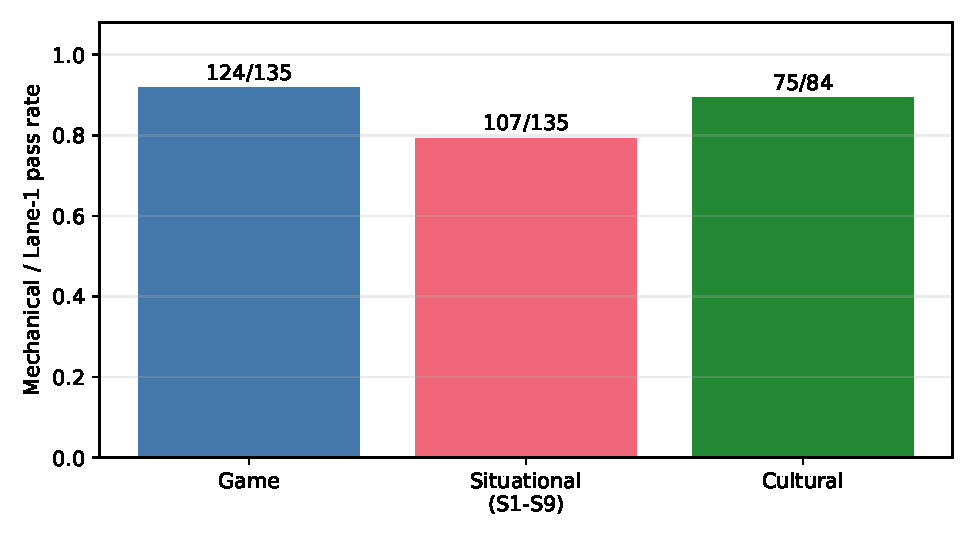
\includegraphics[width=\columnwidth]{fig/three_track_summary.pdf}
    \caption{Mechanical/Lane-1 pass rates for the completed subset of each track. Different formats and evaluators make these descriptive track summaries, not a controlled ranking of task difficulty.}
    \label{fig:three_tracks}
\end{figure}

Together, the three tracks contain 354 first-pass candidates over 32 distinct scenarios. Table~\ref{tab:tracks} keeps the evidence regimes separate: games have formal references, situational cases have executable validation but no unique semantic target, and cultural cases use JSON plus automated diagnostics.

\subsection{Game track: mechanical validity and repair}
Across all trials, 124/135 (91.85\%) succeed on the first attempt. Recorded repair rounds produce a contract-valid final artifact for 135/135 trials. A separate post-hoc Lane-1 audit passes 134/135; the sole failure is DeepSeek G9 in run 1. These quantities answer different questions: first-pass validity measures unaided generation, repair-assisted validity measures the complete generation pipeline, and Lane 1 is a later stricter audit.

\begin{table*}[t]
\centering
\small
\caption{Mechanical reliability and fallback structural comparison over 27 trials per model. Structural values are means; $\pm$ is sample standard deviation across model--game--run rows.}
\label{tab:main_results}
\begin{tabular}{lrrrrrr}
\toprule
Model & First pass & Lane 1 & Coverage & Precision & Structural F1 & Exact \\
\midrule
Claude Opus 5 & 27/27 & 27/27 & .9083 & .4112 & $.5175\pm.3101$ & 1/27 \\
DeepSeek V4 Flash & 23/27 & 26/27 & .7788 & .7334 & $.7071\pm.2868$ & 4/27 \\
GPT-5.6 Sol & 26/27 & 27/27 & .9440 & .7625 & $.7854\pm.3043$ & 11/27 \\
Llama 3.3 70B & 22/27 & 27/27 & .8891 & .7018 & $.7487\pm.2338$ & 9/27 \\
Qwen 3.8 27B & 26/27 & 27/27 & .8577 & .8762 & $.8221\pm.2507$ & 7/27 \\
\bottomrule
\end{tabular}
\end{table*}

\begin{figure}[t]
    \centering
    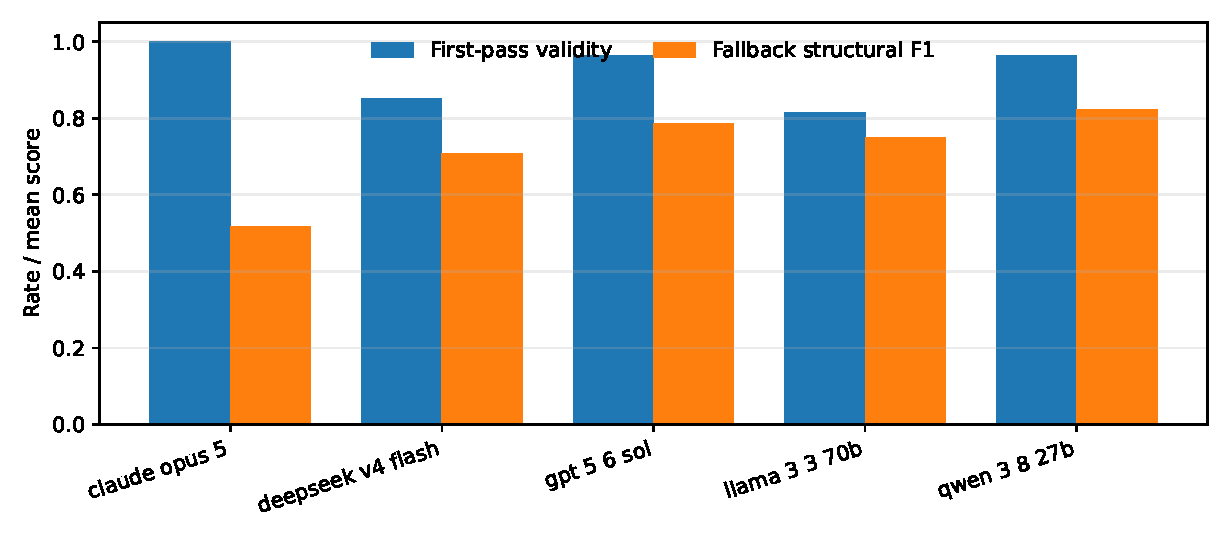
\includegraphics[width=\columnwidth]{fig/main_empirical_results.pdf}
    \caption{First-pass mechanical validity and mean fallback structural F1 by model (27 trials each). Validity is a pass rate; structural F1 is a representation-sensitive feature comparison. Their separation is the central empirical result.}
    \label{fig:main_empirical}
\end{figure}

\subsection{Structural fidelity conditional on validity}
The mean fallback structural F1 over all 135 artifacts is 0.7162. Among the 134 Lane-1-passing artifacts it is 0.7178, and only 32/134 attain F1=1 under the fallback. Thus, the mechanical gate removes almost none of the observed structural variation. Table~\ref{tab:main_results} also shows that coverage alone is insufficient: high coverage can accompany low precision, consistent with extra represented features or finer modeling granularity. We do not label every feature difference an error without case-level semantic inspection.

\subsection{Observed run-to-run reliability}
First-pass validity is 43/45 (95.56\%) in run 1, 41/45 (91.11\%) in run 2, and 40/45 (88.89\%) in run 3. By model it ranges from 22/27 (81.48\%) for Llama to 27/27 (100\%) for Claude; DeepSeek reaches 23/27 and GPT and Qwen each reach 26/27. Three repetitions establish observed variation, not statistical significance or a stable population ranking. The structural standard deviations in Table~\ref{tab:main_results} also mix game difficulty with run variation and are not pure stability estimates.

\begin{table}[t]
\centering
\small
\caption{Game-track reliability by repeated run. ``Final'' includes explicitly recorded repair rounds; attempts counts every first pass and repair call.}
\label{tab:game_runs}
\begin{tabular}{lrrr}
\toprule
Run & First-pass valid & Final valid & Attempts \\
\midrule
1 & 43/45 (95.56\%) & 45/45 & 47 \\
2 & 41/45 (91.11\%) & 45/45 & 50 \\
3 & 40/45 (88.89\%) & 45/45 & 68 \\
\midrule
All & 124/135 (91.85\%) & 135/135 & 165 \\
\bottomrule
\end{tabular}
\end{table}

\subsection{Situational track: executable Python POSGs}
Across the balanced S1--S9 subset, 114/135 first-pass programs execute, 110/135 pass the notebook's validation stage, and 107/135 pass the complete mechanical verdict. Claude and GPT each pass 27/27, Llama 20/27, Qwen 17/27, and DeepSeek 16/27. These rates come directly from saved notebook output rather than from the presence of source files. Repair files are retained but excluded from the headline. The spread is larger than in the game track, consistent with the situational cases' longer, less tightly specified dynamics, but the experiment does not isolate which property causes the difference.

\begin{table}[t]
\centering
\small
\caption{Situational S1--S9 first-pass funnel (three generations per model--case pair). S10--S11 are excluded because their saved execution log is incomplete.}
\label{tab:situational}
\begin{tabular}{lrrr}
\toprule
Model & Executes & Validates & Mechanical pass \\
\midrule
Claude Opus 5 & 27/27 & 27/27 & 27/27 (100\%) \\
GPT-5.6 Sol & 27/27 & 27/27 & 27/27 (100\%) \\
Llama 3.3 70B & 25/27 & 22/27 & 20/27 (74.07\%) \\
Qwen 3.8 27B & 19/27 & 18/27 & 17/27 (62.96\%) \\
DeepSeek V4 Flash & 16/27 & 16/27 & 16/27 (59.26\%) \\
\midrule
All & 114/135 & 110/135 & 107/135 (79.26\%) \\
\bottomrule
\end{tabular}
\end{table}

\subsection{Cultural track: context and semantic diagnostics}
The cultural track has 84 candidates. Strict parsing succeeds for 52/84; documented fence/brace recovery produces parseable candidates for 82/84, and 75/84 pass Lane 1. By run, GPT and Claude each pass Lane 1 on all 28 candidates. Llama passes 8/14 anonymized and 11/14 country-named candidates. Mean fallback structural F1 is 0.6386 versus 0.5777 for GPT, 0.6449 versus 0.6554 for Llama, and 0.4187 versus 0.3977 for Claude (anonymized versus location named).

Mean automated semantic scores change by $-0.006$, $-0.007$, and $-0.001$ when location is revealed for GPT, Llama, and Claude respectively. These are descriptive diagnostics: providers differ for Llama across conditions, there is one sample per cell, reference wording differs slightly in six bullets, and no completed human study validates the automated semantic or bias checks. In particular, diagnostic bias flags are not evidence that a model is biased.

\begin{table*}[t]
\centering
\small
\caption{Cultural-track results by model and prompt condition (14 cases per row). ``Recovered'' denotes documented fence/brace recovery after strict parsing; semantic scores are automated diagnostics, not human judgments.}
\label{tab:cultural}
\begin{tabular}{llrrrrr}
\toprule
Model & Condition & Strict & Recovered & Lane 1 & Structural F1 & Semantic \\
\midrule
GPT-5.6 Sol & Anonymized & 13/14 & 1 & 14/14 & .6386 & .9454 \\
GPT-5.6 Sol & Country named & 13/14 & 1 & 14/14 & .5777 & .9393 \\
Llama 3.3 70B & Anonymized & 0/14 & 12 & 8/14 & .6449 & .8380 \\
Llama 3.3 70B & Country named & 0/14 & 14 & 11/14 & .6554 & .8307 \\
Claude Opus 5 & Anonymized & 13/14 & 1 & 14/14 & .4187 & .9086 \\
Claude Opus 5 & Country named & 13/14 & 1 & 14/14 & .3977 & .9071 \\
\midrule
All & --- & 52/84 & 30 & 75/84 & --- & --- \\
\bottomrule
\end{tabular}
\end{table*}

\section{Discussion and Failure Analysis}
Mechanical correctness is necessary but insufficient for a trustworthy executable world model. In the game track nearly every artifact passes Lane 1, while fallback structural agreement spans a wide range; the other tracks show that even the mechanical gate itself becomes less reliable as scenarios and output regimes change. Differences can reflect under-modeling (missing features or shortened trajectories), over-modeling (extra states or finer outcome expansion), transition or terminal differences, or an alternative but valid granularity. Only reference mechanics and targeted semantic review can distinguish these explanations.

This distinction matters for Physical AI even though the present cases are symbolic controls. An omitted successor can make a harmful state appear unreachable; an invented reverse edge can make an irreversible action appear recoverable; and incorrect stochasticity changes risk estimates. The experiments demonstrate the need for formal evaluation, not real-world safety. No downstream planner or controller is evaluated.

\section{Limitations}
The experiments use symbolic POSGs rather than continuous, perceptual physical dynamics. The game study and reported situational subset have three repetitions per model--case pair; the cultural track has one sample per condition. Provider/model versions may change, and Llama's cultural provider differs by condition. Exhaustive rollout is bounded. Lane 2 uses a representation-sensitive fallback because optimal graph matching was unavailable; topology alone does not establish semantic correctness. Human Lane-3 validation is incomplete, so semantic scores and flags remain diagnostic. The situational S10--S11 execution record is incomplete and excluded, while the v3 JSON track was authored offline by hand and is not reported as LLM performance. We do not measure downstream planning, control, empowerment, reversibility, or real-world safety.

\section{Conclusion}
\label{sec:conclusion}
Across three empirical tracks we analyze 354 first-pass candidates: 135 reference-backed games, 135 logged situational Python POSGs, and 84 cultural JSON models. Mechanical validity varies by track and model. In games, repair makes all final artifacts executable, but structural comparison remains below exact agreement for most mechanically valid outputs. Situational generation shows a wider first-pass mechanical spread, while cultural results expose the importance of separating strict formatting, recovered validity, structural diagnostics, and unvalidated semantic criteria. Executability is therefore a gate, not evidence of world-model fidelity. Future work should complete the remaining situational log, add embodied dynamics and human semantic annotation, validate representation-invariant matching, and test downstream policies.


\section{References}
\label{sec:references}

% Papers to be submitted to NeurIPS 2026 must be prepared according to the
% instructions presented here. Papers may only be up to {\bf nine} pages long, including figures. \textbf{Papers that exceed the page limit will not be reviewed (or in any other way considered) for presentation at the conference.}
% Additional pages \emph{containing acknowledgments, references, checklist, and optional technical appendices} do not count as content pages. 


% The margins in 2026 are the same as those in previous years.


% Authors are required to use the NeurIPS \LaTeX{} style files obtainable at the NeurIPS website as indicated below. Please make sure you use the current files and not previous versions. Tweaking the style files may be grounds for desk rejection.


% \subsection{Retrieval of style files}


% The style files for NeurIPS and other conference information are available on the website at
% \begin{center}
%   \url{https://neurips.cc}.
% \end{center}
% % The file \verb+neurips_2026.pdf+ contains these instructions and illustrates the various formatting requirements your NeurIPS paper must satisfy.


% The only supported style file for NeurIPS 2026 is \verb+neurips_2026.sty+, rewritten for \LaTeXe{}. \textbf{Previous style files for \LaTeX{} 2.09,  Microsoft Word, and RTF are no longer supported.}


% The \LaTeX{} style file contains three optional arguments: 
% \begin{itemize}
% \item \verb+final+, which creates a camera-ready copy, 
% \item \verb+preprint+, which creates a preprint for submission to, e.g., arXiv, \item \verb+nonatbib+, which will not load the \verb+natbib+ package for you in case of package clash.
% \end{itemize}


% \paragraph{Preprint option}
% If you wish to post a preprint of your work online, e.g., on arXiv, using the NeurIPS style, please use the \verb+preprint+ option. This will create a nonanonymized version of your work with the text ``Preprint. Work in progress.'' in the footer. This version may be distributed as you see fit, as long as you do not say which conference it was submitted to. Please \textbf{do not} use the \verb+final+ option, which should \textbf{only} be used for papers accepted to NeurIPS.


% At submission time, please omit the \verb+final+ and \verb+preprint+ options. This will anonymize your submission and add line numbers to aid review. Please do \emph{not} refer to these line numbers in your paper as they will be removed during generation of camera-ready copies.


% The file \verb+neurips_2026.tex+ may be used as a ``shell'' for writing your paper. All you have to do is replace the author, title, abstract, and text of the paper with your own.


% The formatting instructions contained in these style files are summarized in Sections \ref{gen_inst}, \ref{headings}, and \ref{others} below.


% \section{General formatting instructions}
% \label{gen_inst}


% The text must be confined within a rectangle 5.5~inches (33~picas) wide and
% 9~inches (54~picas) long. The left margin is 1.5~inch (9~picas).  Use 10~point
% type with a vertical spacing (leading) of 11~points.  Times New Roman is the
% preferred typeface throughout, and will be selected for you by default.
% Paragraphs are separated by \nicefrac{1}{2}~line space (5.5 points), with no
% indentation.


% The paper title should be 17~point, initial caps/lower case, bold, centered
% between two horizontal rules. The top rule should be 4~points thick and the
% bottom rule should be 1~point thick. Allow \nicefrac{1}{4}~inch space above and
% below the title to rules. All pages should start at 1~inch (6~picas) from the
% top of the page.


% For the final version, authors' names are set in boldface, and each name is
% centered above the corresponding address. The lead author's name is to be listed
% first (left-most), and the co-authors' names (if different address) are set to
% follow. If there is only one co-author, list both author and co-author side by
% side.


% Please pay special attention to the instructions in Section \ref{others}
% regarding figures, tables, acknowledgments, and references.

% \section{Headings: first level}
% \label{headings}


% All headings should be lower case (except for first word and proper nouns),
% flush left, and bold.


% First-level headings should be in 12-point type.


% \subsection{Headings: second level}


% Second-level headings should be in 10-point type.


% \subsubsection{Headings: third level}


% Third-level headings should be in 10-point type.


% \paragraph{Paragraphs}


% There is also a \verb+\paragraph+ command available, which sets the heading in
% bold, flush left, and inline with the text, with the heading followed by 1\,em
% of space.


% \section{Citations, figures, tables, references}
% \label{others}


% These instructions apply to everyone.


% \subsection{Citations within the text}


% The \verb+natbib+ package will be loaded for you by default.  Citations may be
% author/year or numeric, as long as you maintain internal consistency.  As to the
% format of the references themselves, any style is acceptable as long as it is
% used consistently.


% The documentation for \verb+natbib+ may be found at
% \begin{center}
%   \url{http://mirrors.ctan.org/macros/latex/contrib/natbib/natnotes.pdf}
% \end{center}
% Of note is the command \verb+\citet+, which produces citations appropriate for
% use in inline text.  For example,
% \begin{verbatim}
%    \citet{hasselmo} investigated\dots
% \end{verbatim}
% produces
% \begin{quote}
%   Hasselmo, et al.\ (1995) investigated\dots
% \end{quote}


% If you wish to load the \verb+natbib+ package with options, you may add the
% following before loading the \verb+neurips_2026+ package:
% \begin{verbatim}
%    \PassOptionsToPackage{options}{natbib}
% \end{verbatim}


% If \verb+natbib+ clashes with another package you load, you can add the optional
% argument \verb+nonatbib+ when loading the style file:
% \begin{verbatim}
%    \usepackage[nonatbib]{neurips_2026}
% \end{verbatim}


% As submission is double blind, refer to your own published work in the third
% person. That is, use ``In the previous work of Jones et al.\ [4],'' not ``In our
% previous work [4].'' If you cite your other papers that are not widely available
% (e.g., a journal paper under review), use anonymous author names in the
% citation, e.g., an author of the form ``A.\ Anonymous'' and include a copy of the anonymized paper in the supplementary material.


% \subsection{Footnotes}


% Footnotes should be used sparingly.  If you do require a footnote, indicate
% footnotes with a number\footnote{Sample of the first footnote.} in the
% text. Place the footnotes at the bottom of the page on which they appear.
% Precede the footnote with a horizontal rule of 2~inches (12~picas).


% Note that footnotes are properly typeset \emph{after} punctuation
% marks.\footnote{As in this example.}


% \subsection{Figures}


% \begin{figure}
%   \centering
%   \fbox{\rule[-.5cm]{0cm}{4cm} \rule[-.5cm]{4cm}{0cm}}
%   \caption{Sample figure caption. Explain what the figure shows and add a key take-away message to the caption.}
% \end{figure}


% All artwork must be neat, clean, and legible. Lines should be dark enough for
%  reproduction purposes. The figure number and caption always appear after the
% figure. Place one line space before the figure caption and one line space after
% the figure. The figure caption should be lower case (except for the first word and proper nouns); figures are numbered consecutively.


% You may use color figures.  However, it is best for the figure captions and the
% paper body to be legible if the paper is printed in either black/white or in
% color.


% \subsection{Tables}


% All tables must be centered, neat, clean, and legible.  The table number and
% title always appear before the table.  See Table~\ref{sample-table}.


% Place one line space before the table title, one line space after the
% table title, and one line space after the table. The table title must
% be lower case (except for the first word and proper nouns); tables are
% numbered consecutively.


% Note that publication-quality tables \emph{do not contain vertical rules}. We
% strongly suggest the use of the \verb+booktabs+ package, which allows for
% typesetting high-quality, professional tables:
% \begin{center}
%   \url{https://www.ctan.org/pkg/booktabs}
% \end{center}
% This package was used to typeset Table~\ref{sample-table}.


% \begin{table}
%   \caption{Sample table caption. Explain what the table shows and add a key take-away message to the caption.}
%   \label{sample-table}
%   \centering
%   \begin{tabular}{lll}
%     \toprule
%     \multicolumn{2}{c}{Part}                   \\
%     \cmidrule(r){1-2}
%     Name     & Description     & Size ($\mu$m) \\
%     \midrule
%     Dendrite & Input terminal  & $\approx$100     \\
%     Axon     & Output terminal & $\approx$10      \\
%     Soma     & Cell body       & up to $10^6$  \\
%     \bottomrule
%   \end{tabular}
% \end{table}

% \subsection{Math}
% Note that display math in bare TeX commands will not create correct line numbers for submission. Please use LaTeX (or AMSTeX) commands for unnumbered display math. (You really shouldn't be using \$\$ anyway; see \url{https://tex.stackexchange.com/questions/503/why-is-preferable-to} and \url{https://tex.stackexchange.com/questions/40492/what-are-the-differences-between-align-equation-and-displaymath} for more information.)

% \subsection{Final instructions}

% Do not change any aspects of the formatting parameters in the style files.  In
% particular, do not modify the width or length of the rectangle the text should
% fit into, and do not change font sizes. Please note that pages should be
% numbered.


% \section{Preparing PDF files}


% Please prepare submission files with paper size ``US Letter,'' and not, for
% example, ``A4.''


% Fonts were the main cause of problems in the past years. Your PDF file must only
% contain Type 1 or Embedded TrueType fonts. Here are a few instructions to
% achieve this.


% \begin{itemize}


% \item You should directly generate PDF files using \verb+pdflatex+.


% \item You can check which fonts a PDF files uses.  In Acrobat Reader, select the
%   menu Files$>$Document Properties$>$Fonts and select Show All Fonts. You can
%   also use the program \verb+pdffonts+ which comes with \verb+xpdf+ and is
%   available out-of-the-box on most Linux machines.


% \item \verb+xfig+ ``patterned'' shapes are implemented with bitmap fonts.  Use
%   "solid" shapes instead.


% \item The \verb+\bbold+ package almost always uses bitmap fonts.  You should use
%   the equivalent AMS Fonts:
% \begin{verbatim}
%    \usepackage{amsfonts}
% \end{verbatim}
% followed by, e.g., \verb+\mathbb{R}+, \verb+\mathbb{N}+, or \verb+\mathbb{C}+
% for $\mathbb{R}$, $\mathbb{N}$ or $\mathbb{C}$.  You can also use the following
% workaround for reals, natural and complex:
% \begin{verbatim}
%    \newcommand{\RR}{I\!\!R} %real numbers
%    \newcommand{\Nat}{I\!\!N} %natural numbers
%    \newcommand{\CC}{I\!\!\!\!C} %complex numbers
% \end{verbatim}
% Note that \verb+amsfonts+ is automatically loaded by the \verb+amssymb+ package.


% \end{itemize}


% If your file contains type 3 fonts or non embedded TrueType fonts, we will ask
% you to fix it.


% \subsection{Margins in \LaTeX{}}


% Most of the margin problems come from figures positioned by hand using
% \verb+\special+ or other commands. We suggest using the command
% \verb+\includegraphics+ from the \verb+graphicx+ package. Always specify the
% figure width as a multiple of the line width as in the example below:
% \begin{verbatim}
%    \usepackage[pdftex]{graphicx} ...
%    \includegraphics[width=0.8\linewidth]{myfile.pdf}
% \end{verbatim}
% See Section 4.4 in the graphics bundle documentation
% (\url{http://mirrors.ctan.org/macros/latex/required/graphics/grfguide.pdf})


% A number of width problems arise when \LaTeX{} cannot properly hyphenate a
% line. Please give LaTeX hyphenation hints using the \verb+\-+ command when
% necessary.

% \begin{ack}
% Use unnumbered first level headings for the acknowledgments. All acknowledgments
% go at the end of the paper before the list of references. Moreover, you are required to declare
% funding (financial activities supporting the submitted work) and competing interests (related financial activities outside the submitted work).
% More information about this disclosure can be found at: \url{https://neurips.cc/Conferences/2026/PaperInformation/FundingDisclosure}.


% Do {\bf not} include this section in the anonymized submission, only in the final paper. You can use the \texttt{ack} environment provided in the style file to automatically hide this section in the anonymized submission.
% \end{ack}

%\section*{References}
%\bibliographystyle{plainnat}
\bibliographystyle{unsrtnat} 
%\bibliography{reference}

%References follow the acknowledgments in the camera-ready paper. Use unnumbered first-level heading for
%the references. Any choice of citation style is acceptable as long as you are
%consistent. It is permissible to reduce the font size to \verb+small+ (9 point)
%when listing the references.
%Note that the Reference section does not count towards the page limit.
\medskip


{
\small
\bibliography{reference}

%[1] Alexander, J.A.\ \& Mozer, M.C.\ (1995) Template-based algorithms for connectionist rule extraction. In G.\ Tesauro, D.S.\ Touretzky and T.K.\ Leen (eds.), {\it Advances in Neural Information Processing Systems 7}, pp.\ 609--616. Cambridge, MA: MIT Press.


%[2] Bower, J.M.\ \& Beeman, D.\ (1995) {\it The Book of GENESIS: Exploring Realistic Neural Models with the GEneral NEural SImulation System.}  New York: TELOS/Springer--Verlag.


%[3] Hasselmo, M.E., Schnell, E.\ \& Barkai, E.\ (1995) Dynamics of learning and recall at excitatory recurrent synapses and cholinergic modulation in rat hippocampal region CA3. {\it Journal of Neuroscience} {\bf 15}(7):5249-5262.
}


%%%%%%%%%%%%%%%%%%%%%%%%%%%%%%%%%%%%%%%%%%%%%%%%%%%%%%%%%%%%

\appendix

\section{Additional graph diagnostics}
\subsection{Case-level results}
\begin{table}[h]
\centering
\small
\caption{Game results by case, pooled over five models and three runs (15 candidates per case). F1 is the mean feature-multiset fallback score.}
\label{tab:game_cases}
\begin{tabular}{lrrrrrrrrr}
\toprule
Case & G1 & G2 & G3 & G4 & G5 & G6 & G7 & G8 & G9 \\
\midrule
Lane 1 & 15 & 15 & 15 & 15 & 15 & 15 & 15 & 15 & 14 \\
Mean F1 & .851 & .201 & .756 & .881 & .889 & .449 & .855 & .745 & .819 \\
\bottomrule
\end{tabular}
\end{table}

\begin{table}[h]
\centering
\small
\caption{Situational first-pass mechanical validity by case, pooled over five models and three generations (15 attempts per case).}
\label{tab:situational_cases}
\begin{tabular}{lrrrrrrrrr}
\toprule
Case & S1 & S2 & S3 & S4 & S5 & S6 & S7 & S8 & S9 \\
\midrule
Pass & 13 & 13 & 11 & 10 & 13 & 11 & 12 & 13 & 11 \\
Total & 15 & 15 & 15 & 15 & 15 & 15 & 15 & 15 & 15 \\
\bottomrule
\end{tabular}
\end{table}

\begin{table*}[h]
\centering
\small
\caption{Cultural results by case, pooled over three models and two prompt conditions (six candidates per case). Semantic values are automated diagnostics.}
\label{tab:cultural_cases}
\begin{tabular}{lrrrrrrrrrrrrrr}
\toprule
Case & C1 & C2 & C3 & C4 & C5 & C6 & C7 & C8 & C9 & C10 & C11 & C12 & C13 & C14 \\
\midrule
Lane 1 & 6 & 6 & 6 & 6 & 5 & 6 & 4 & 6 & 5 & 5 & 4 & 4 & 6 & 6 \\
Mean F1 & .676 & .634 & .630 & .595 & .528 & .411 & .377 & .529 & .524 & .546 & .490 & .647 & .461 & .692 \\
Mean semantic & .903 & .909 & .841 & .887 & .963 & .855 & .878 & .856 & .924 & .869 & .898 & .906 & .927 & .938 \\
\bottomrule
\end{tabular}
\end{table*}

Figure~\ref{fig:reference_comparison} characterizes the structural diversity of the nine reference games used by the evaluation. Figure~\ref{fig:qwen_example} records an earlier local-Qwen G1 artifact that passed structural rollout but failed game-specific reward and observation checks. This example is diagnostic and is not pooled with the five-model study.

\begin{figure}[h]
    \centering
    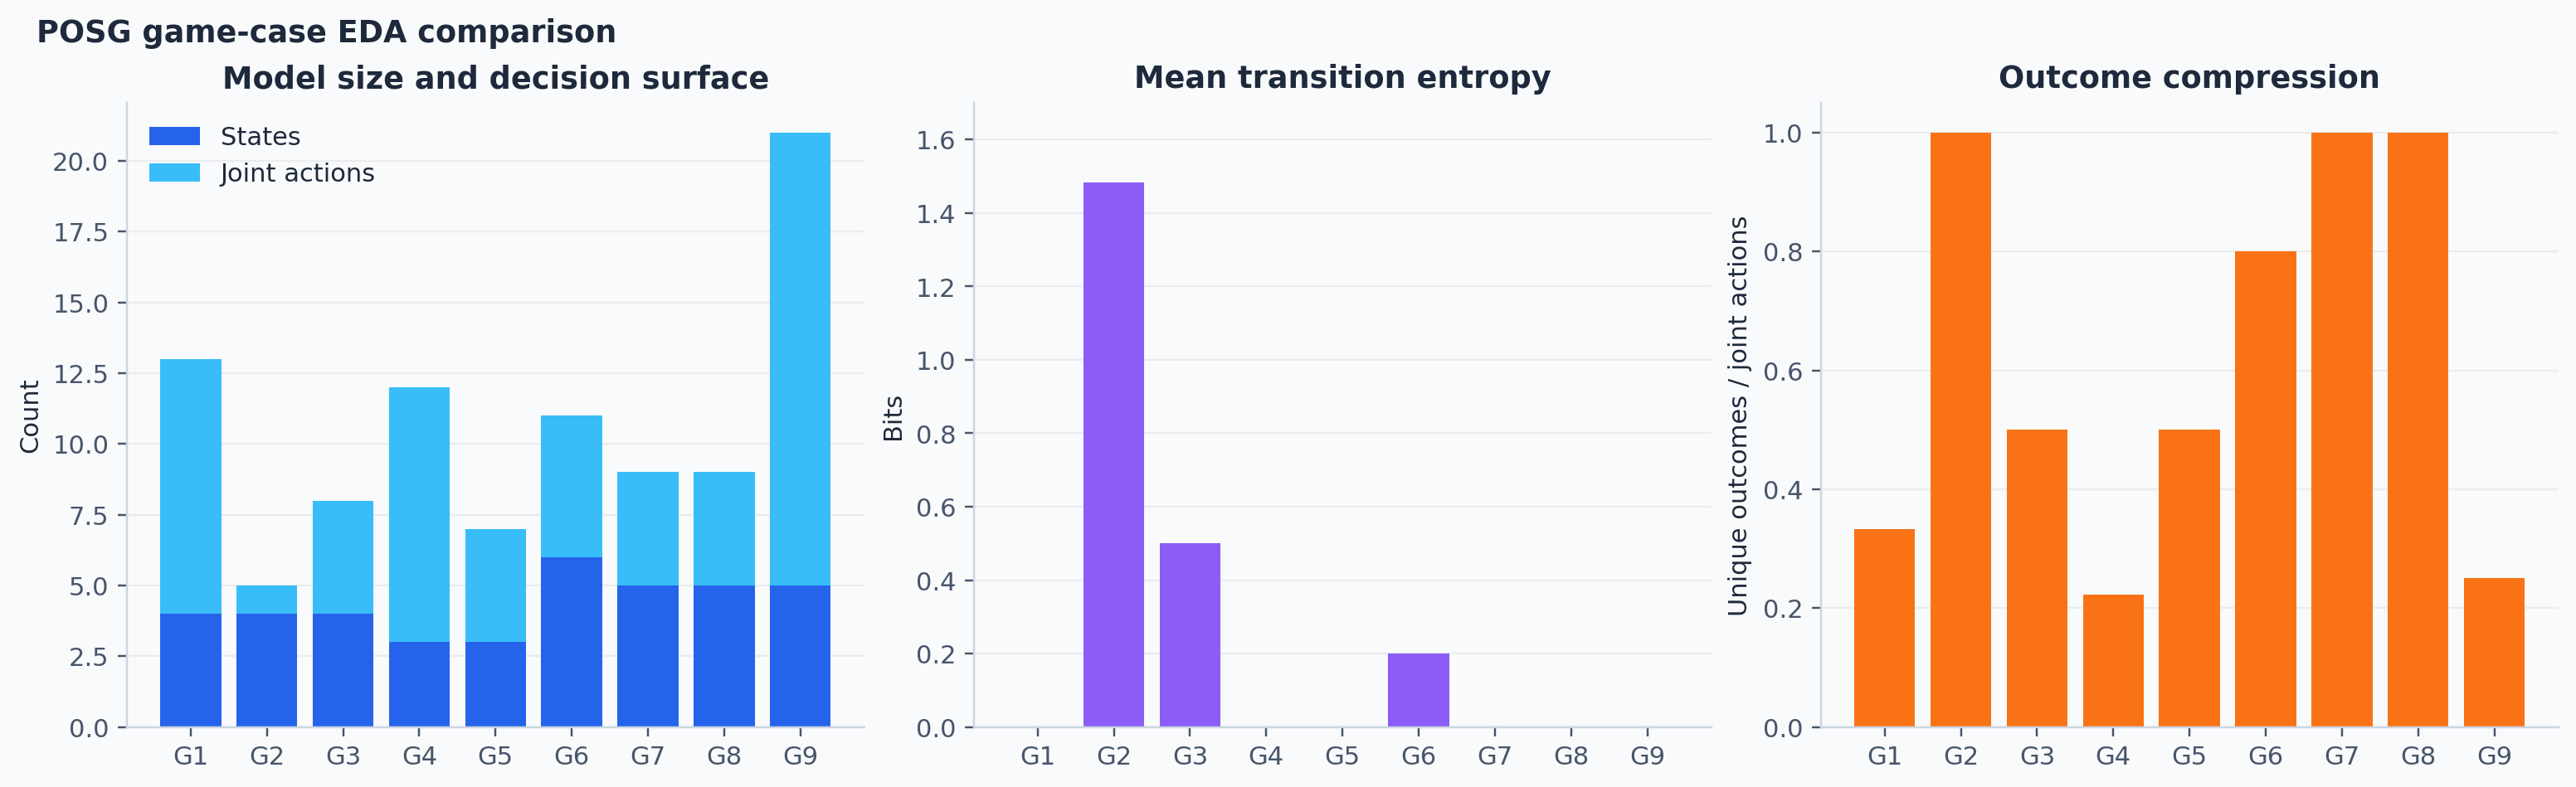
\includegraphics[width=\linewidth]{fig/game_case_comparison.png}
    \caption{Cross-case graph statistics for the G1--G9 reference fixtures. These are controls, not generated-model performance.}
    \label{fig:reference_comparison}
\end{figure}

\begin{figure}[h]
    \centering
    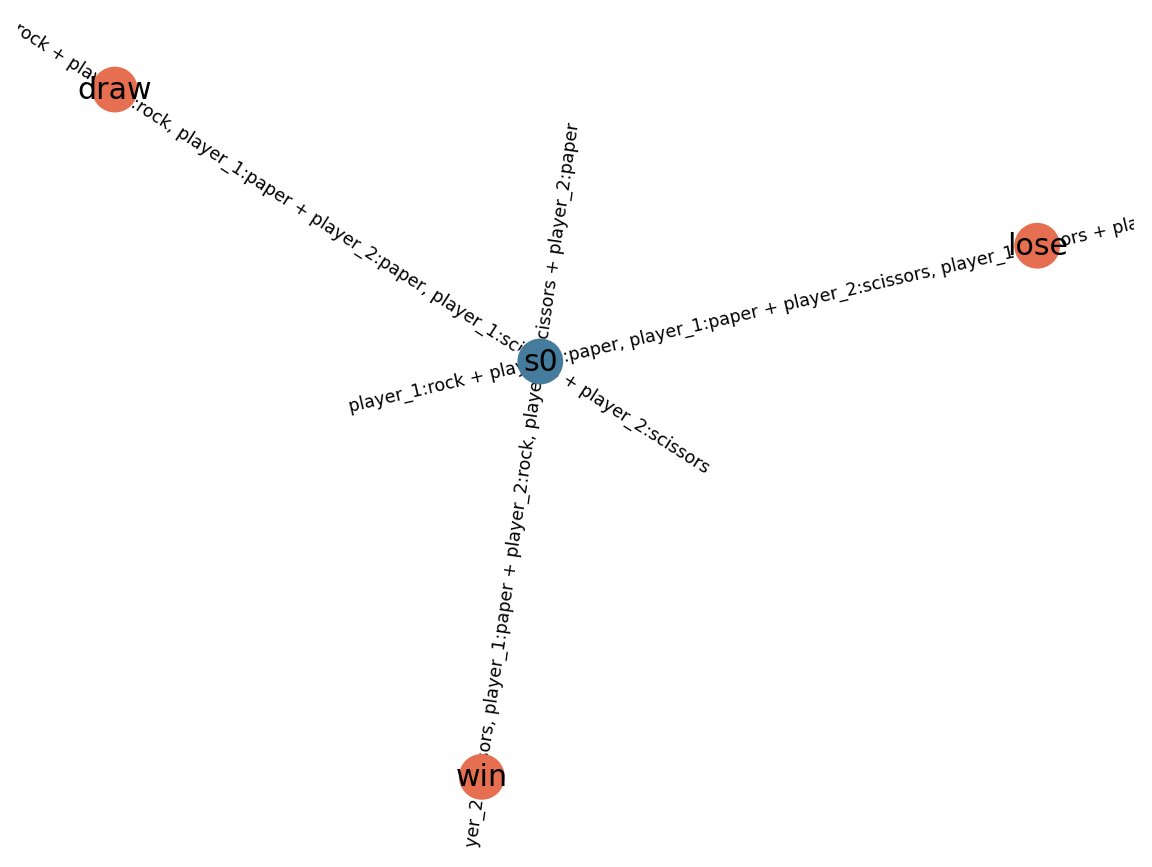
\includegraphics[width=.75\linewidth]{fig/qwen_g1_sample_003_graph.png}
    \caption{State graph for an earlier local-Qwen G1 sample. A plausible graph did not prevent incorrect rewards and player-specific observations, illustrating why topology alone is insufficient.}
    \label{fig:qwen_example}
\end{figure}

%%%%%%%%%%%%%%%%%%%%%%%%%%%%%%%%%%%%%%%%%%%%%%%%%%%%%%%%%%%%

% \todo[inline]{
% Ani: Just commentted out for the time being
% }
\newpage
\section*{NeurIPS Paper Checklist}

%%% BEGIN INSTRUCTIONS %%%
% The checklist is designed to encourage best practices for responsible machine learning research, addressing issues of reproducibility, transparency, research ethics, and societal impact. Do not remove the checklist: {\bf The papers not including the checklist will be desk rejected.} The checklist should follow the references and follow the (optional) supplemental material.  The checklist does NOT count towards the page
% limit. 

% Please read the checklist guidelines carefully for information on how to answer these questions. For each question in the checklist:
% \begin{itemize}
%     \item You should answer \answerYes{}, \answerNo{}, or \answerNA{}.
%     \item \answerNA{} means either that the question is Not Applicable for that particular paper or the relevant information is Not Available.
%     \item Please provide a short (1--2 sentence) justification right after your answer (even for \answerNA). 
%    % \item {\bf The papers not including the checklist will be desk rejected.}
% \end{itemize}

% {\bf The checklist answers are an integral part of your paper submission.} They are visible to the reviewers, area chairs, senior area chairs, and ethics reviewers. You will also be asked to include it (after eventual revisions) with the final version of your paper, and its final version will be published with the paper.

% The reviewers of your paper will be asked to use the checklist as one of the factors in their evaluation. While \answerYes{} is generally preferable to \answerNo{}, it is perfectly acceptable to answer \answerNo{} provided a proper justification is given (e.g., error bars are not reported because it would be too computationally expensive'' or ``we were unable to find the license for the dataset we used''). In general, answering \answerNo{} or \answerNA{} is not grounds for rejection. While the questions are phrased in a binary way, we acknowledge that the true answer is often more nuanced, so please just use your best judgment and write a justification to elaborate. All supporting evidence can appear either in the main paper or the supplemental material, provided in appendix. If you answer \answerYes{} to a question, in the justification please point to the section(s) where related material for the question can be found.

% IMPORTANT, please:
% \begin{itemize}
%     \item {\bf Delete this instruction block, but keep the section heading ``NeurIPS Paper Checklist"},
%     \item  {\bf Keep the checklist subsection headings, questions/answers and guidelines below.}
%     \item {\bf Do not modify the questions and only use the provided macros for your answers}.
% \end{itemize} 
 

%%% END INSTRUCTIONS %%%


\begin{enumerate}

\item {\bf Claims}
    \item[] Question: Do the main claims made in the abstract and introduction accurately reflect the paper's contributions and scope?
    \item[] Answer: \answerYes{} % Replace by \answerYes{}, \answerNo{}, or \answerNA{}.
    \item[] Justification: 
    The abstract and Introduction state the scope of the work as generating and evaluating LLM produced situational world models represented as stochastic games, and describe the benchmark, generation pipeline, and multi-lane evaluation framework.

    
    \item[] Guidelines:
    \begin{itemize}
        \item The answer \answerNA{} means that the abstract and introduction do not include the claims made in the paper.
        \item The abstract and/or introduction should clearly state the claims made, including the contributions made in the paper and important assumptions and limitations. A \answerNo{} or \answerNA{} answer to this question will not be perceived well by the reviewers. 
        \item The claims made should match theoretical and experimental results, and reflect how much the results can be expected to generalize to other settings. 
        \item It is fine to include aspirational goals as motivation as long as it is clear that these goals are not attained by the paper. 
    \end{itemize}

\item {\bf Limitations}
    \item[] Question: Does the paper discuss the limitations of the work performed by the authors?
    \item[] Answer: \answerYes{} % Replace by \answerYes{}, \answerNo{}, or \answerNA{}.
    \item[] Justification: We clarify this is work in progress and experimental validation is ongoing
    \item[] Guidelines:
    \begin{itemize}
        \item The answer \answerNA{} means that the paper has no limitation while the answer \answerNo{} means that the paper has limitations, but those are not discussed in the paper. 
        \item The authors are encouraged to create a separate ``Limitations'' section in their paper.
        \item The paper should point out any strong assumptions and how robust the results are to violations of these assumptions (e.g., independence assumptions, noiseless settings, model well-specification, asymptotic approximations only holding locally). The authors should reflect on how these assumptions might be violated in practice and what the implications would be.
        \item The authors should reflect on the scope of the claims made, e.g., if the approach was only tested on a few datasets or with a few runs. In general, empirical results often depend on implicit assumptions, which should be articulated.
        \item The authors should reflect on the factors that influence the performance of the approach. For example, a facial recognition algorithm may perform poorly when image resolution is low or images are taken in low lighting. Or a speech-to-text system might not be used reliably to provide closed captions for online lectures because it fails to handle technical jargon.
        \item The authors should discuss the computational efficiency of the proposed algorithms and how they scale with dataset size.
        \item If applicable, the authors should discuss possible limitations of their approach to address problems of privacy and fairness.
        \item While the authors might fear that complete honesty about limitations might be used by reviewers as grounds for rejection, a worse outcome might be that reviewers discover limitations that aren't acknowledged in the paper. The authors should use their best judgment and recognize that individual actions in favor of transparency play an important role in developing norms that preserve the integrity of the community. Reviewers will be specifically instructed to not penalize honesty concerning limitations.
    \end{itemize}

\item {\bf Theory assumptions and proofs}
    \item[] Question: For each theoretical result, does the paper provide the full set of assumptions and a complete (and correct) proof?
    \item[] Answer: \answerNA{} % Replace by \answerYes{}, \answerNo{}, or \answerNA{}.
    \item[] Justification: 
    The paper does not introduce new theoretical results, theorems, or proofs. Formal definitions are used only to specify the stochastic-game representation and evaluation setting.
    
    \item[] Guidelines:
    \begin{itemize}
        \item The answer \answerNA{} means that the paper does not include theoretical results. 
        \item All the theorems, formulas, and proofs in the paper should be numbered and cross-referenced.
        \item All assumptions should be clearly stated or referenced in the statement of any theorems.
        \item The proofs can either appear in the main paper or the supplemental material, but if they appear in the supplemental material, the authors are encouraged to provide a short proof sketch to provide intuition. 
        \item Inversely, any informal proof provided in the core of the paper should be complemented by formal proofs provided in appendix or supplemental material.
        \item Theorems and Lemmas that the proof relies upon should be properly referenced. 
    \end{itemize}

    \item {\bf Experimental result reproducibility}
    \item[] Question: Does the paper fully disclose all the information needed to reproduce the main experimental results of the paper to the extent that it affects the main claims and/or conclusions of the paper (regardless of whether the code and data are provided or not)?
    \item[] Answer: \answerYes{} % Replace by \answerYes{}, \answerNo{}, or \answerNA{}.
    \item[] Justification: 
    The paper and supplementary material specify the evaluated models, prompts, test cases, validation procedure, and evaluation methodology. Code, prompts, generated outputs, and experiment configurations are provided to enable replication of the reported results.
    
    \item[] Guidelines:
    \begin{itemize}
        \item The answer \answerNA{} means that the paper does not include experiments.
        \item If the paper includes experiments, a \answerNo{} answer to this question will not be perceived well by the reviewers: Making the paper reproducible is important, regardless of whether the code and data are provided or not.
        \item If the contribution is a dataset and\slash or model, the authors should describe the steps taken to make their results reproducible or verifiable. 
        \item Depending on the contribution, reproducibility can be accomplished in various ways. For example, if the contribution is a novel architecture, describing the architecture fully might suffice, or if the contribution is a specific model and empirical evaluation, it may be necessary to either make it possible for others to replicate the model with the same dataset, or provide access to the model. In general. releasing code and data is often one good way to accomplish this, but reproducibility can also be provided via detailed instructions for how to replicate the results, access to a hosted model (e.g., in the case of a large language model), releasing of a model checkpoint, or other means that are appropriate to the research performed.
        \item While NeurIPS does not require releasing code, the conference does require all submissions to provide some reasonable avenue for reproducibility, which may depend on the nature of the contribution. For example
        \begin{enumerate}
            \item If the contribution is primarily a new algorithm, the paper should make it clear how to reproduce that algorithm.
            \item If the contribution is primarily a new model architecture, the paper should describe the architecture clearly and fully.
            \item If the contribution is a new model (e.g., a large language model), then there should either be a way to access this model for reproducing the results or a way to reproduce the model (e.g., with an open-source dataset or instructions for how to construct the dataset).
            \item We recognize that reproducibility may be tricky in some cases, in which case authors are welcome to describe the particular way they provide for reproducibility. In the case of closed-source models, it may be that access to the model is limited in some way (e.g., to registered users), but it should be possible for other researchers to have some path to reproducing or verifying the results.
        \end{enumerate}
    \end{itemize}


\item {\bf Open access to data and code}
    \item[] Question: Does the paper provide open access to the data and code, with sufficient instructions to faithfully reproduce the main experimental results, as described in supplemental material?
    \item[] Answer: \answerYes{} % Replace by \answerYes{}, \answerNo{}, or \answerNA{}.
    \item[] Justification: 
    The repository provided includes instructions for reproducing the generation and evaluation pipeline.
    
    \item[] Guidelines:
    \begin{itemize}
        \item The answer \answerNA{} means that paper does not include experiments requiring code.
        \item Please see the NeurIPS code and data submission guidelines (\url{https://neurips.cc/public/guides/CodeSubmissionPolicy}) for more details.
        \item While we encourage the release of code and data, we understand that this might not be possible, so \answerNo{} is an acceptable answer. Papers cannot be rejected simply for not including code, unless this is central to the contribution (e.g., for a new open-source benchmark).
        \item The instructions should contain the exact command and environment needed to run to reproduce the results. See the NeurIPS code and data submission guidelines (\url{https://neurips.cc/public/guides/CodeSubmissionPolicy}) for more details.
        \item The authors should provide instructions on data access and preparation, including how to access the raw data, preprocessed data, intermediate data, and generated data, etc.
        \item The authors should provide scripts to reproduce all experimental results for the new proposed method and baselines. If only a subset of experiments are reproducible, they should state which ones are omitted from the script and why.
        \item At submission time, to preserve anonymity, the authors should release anonymized versions (if applicable).
        \item Providing as much information as possible in supplemental material (appended to the paper) is recommended, but including URLs to data and code is permitted.
    \end{itemize}


\item {\bf Experimental setting/details}
    \item[] Question: Does the paper specify all the training and test details (e.g., data splits, hyperparameters, how they were chosen, type of optimizer) necessary to understand the results?
    \item[] Answer: \answerNA{} % Replace by \answerYes{}, \answerNo{}, or \answerNA{}.
    \item[] Justification: 
    The paper does not report experimental results requiring training or test settings. It presents the benchmark, world-model generation pipeline, and evaluation methodology.
    
    \item[] Guidelines:
    \begin{itemize}
        \item The answer \answerNA{} means that the paper does not include experiments.
        \item The experimental setting should be presented in the core of the paper to a level of detail that is necessary to appreciate the results and make sense of them.
        \item The full details can be provided either with the code, in appendix, or as supplemental material.
    \end{itemize}

\item {\bf Experiment statistical significance}
    \item[] Question: Does the paper report error bars suitably and correctly defined or other appropriate information about the statistical significance of the experiments?
    \item[] Answer: \answerNA{} % Replace by \answerYes{}, \answerNo{}, or \answerNA{}.
    \item[] Justification: No experiments were reported.
    \item[] Guidelines:
    \begin{itemize}
        \item The answer \answerNA{} means that the paper does not include experiments.
        \item The authors should answer \answerYes{} if the results are accompanied by error bars, confidence intervals, or statistical significance tests, at least for the experiments that support the main claims of the paper.
        \item The factors of variability that the error bars are capturing should be clearly stated (for example, train/test split, initialization, random drawing of some parameter, or overall run with given experimental conditions).
        \item The method for calculating the error bars should be explained (closed form formula, call to a library function, bootstrap, etc.)
        \item The assumptions made should be given (e.g., Normally distributed errors).
        \item It should be clear whether the error bar is the standard deviation or the standard error of the mean.
        \item It is OK to report 1-sigma error bars, but one should state it. The authors should preferably report a 2-sigma error bar than state that they have a 96\% CI, if the hypothesis of Normality of errors is not verified.
        \item For asymmetric distributions, the authors should be careful not to show in tables or figures symmetric error bars that would yield results that are out of range (e.g., negative error rates).
        \item If error bars are reported in tables or plots, the authors should explain in the text how they were calculated and reference the corresponding figures or tables in the text.
    \end{itemize}

\item {\bf Experiments compute resources}
    \item[] Question: For each experiment, does the paper provide sufficient information on the computer resources (type of compute workers, memory, time of execution) needed to reproduce the experiments?
    \item[] Answer: \answerNA{} % Replace by \answerYes{}, \answerNo{}, or \answerNA{}.
    \item[] Justification: No experiments were reported.
    \item[] Guidelines:
    \begin{itemize}
        \item The answer \answerNA{} means that the paper does not include experiments.
        \item The paper should indicate the type of compute workers CPU or GPU, internal cluster, or cloud provider, including relevant memory and storage.
        \item The paper should provide the amount of compute required for each of the individual experimental runs as well as estimate the total compute. 
        \item The paper should disclose whether the full research project required more compute than the experiments reported in the paper (e.g., preliminary or failed experiments that didn't make it into the paper). 
    \end{itemize}
    
\item {\bf Code of ethics}
    \item[] Question: Does the research conducted in the paper conform, in every respect, with the NeurIPS Code of Ethics \url{https://neurips.cc/public/EthicsGuidelines}?
    \item[] Answer: \answerYes{} % Replace by \answerYes{}, \answerNo{}, or \answerNA{}.
    \item[] Justification: We do not use any human data in this paper.
    \item[] Guidelines:
    \begin{itemize}
        \item The answer \answerNA{} means that the authors have not reviewed the NeurIPS Code of Ethics.
        \item If the authors answer \answerNo, they should explain the special circumstances that require a deviation from the Code of Ethics.
        \item The authors should make sure to preserve anonymity (e.g., if there is a special consideration due to laws or regulations in their jurisdiction).
    \end{itemize}


\item {\bf Broader impacts}
    \item[] Question: Does the paper discuss both potential positive societal impacts and negative societal impacts of the work performed?
    \item[] Answer: \answerNA{} % Replace by \answerYes{}, \answerNo{}, or \answerNA{}.
    \item[] Justification: We don't think the work has societal impact at this point. In the long run, this research agenda should of course help reducing biases and risks in AI decision making.
    \item[] Guidelines:
    \begin{itemize}
        \item The answer \answerNA{} means that there is no societal impact of the work performed.
        \item If the authors answer \answerNA{} or \answerNo, they should explain why their work has no societal impact or why the paper does not address societal impact.
        \item Examples of negative societal impacts include potential malicious or unintended uses (e.g., disinformation, generating fake profiles, surveillance), fairness considerations (e.g., deployment of technologies that could make decisions that unfairly impact specific groups), privacy considerations, and security considerations.
        \item The conference expects that many papers will be foundational research and not tied to particular applications, let alone deployments. However, if there is a direct path to any negative applications, the authors should point it out. For example, it is legitimate to point out that an improvement in the quality of generative models could be used to generate Deepfakes for disinformation. On the other hand, it is not needed to point out that a generic algorithm for optimizing neural networks could enable people to train models that generate Deepfakes faster.
        \item The authors should consider possible harms that could arise when the technology is being used as intended and functioning correctly, harms that could arise when the technology is being used as intended but gives incorrect results, and harms following from (intentional or unintentional) misuse of the technology.
        \item If there are negative societal impacts, the authors could also discuss possible mitigation strategies (e.g., gated release of models, providing defenses in addition to attacks, mechanisms for monitoring misuse, mechanisms to monitor how a system learns from feedback over time, improving the efficiency and accessibility of ML).
    \end{itemize}
    
\item {\bf Safeguards}
    \item[] Question: Does the paper describe safeguards that have been put in place for responsible release of data or models that have a high risk for misuse (e.g., pre-trained language models, image generators, or scraped datasets)?
    \item[] Answer: \answerNA{} % Replace by \answerYes{}, \answerNo{}, or \answerNA{}.
    \item[] Justification: We can think of no way the current work poses such risks
    \item[] Guidelines:
    \begin{itemize}
        \item The answer \answerNA{} means that the paper poses no such risks.
        \item Released models that have a high risk for misuse or dual-use should be released with necessary safeguards to allow for controlled use of the model, for example by requiring that users adhere to usage guidelines or restrictions to access the model or implementing safety filters. 
        \item Datasets that have been scraped from the Internet could pose safety risks. The authors should describe how they avoided releasing unsafe images.
        \item We recognize that providing effective safeguards is challenging, and many papers do not require this, but we encourage authors to take this into account and make a best faith effort.
    \end{itemize}

\item {\bf Licenses for existing assets}
    \item[] Question: Are the creators or original owners of assets (e.g., code, data, models), used in the paper, properly credited and are the license and terms of use explicitly mentioned and properly respected?
    \item[] Answer: \answerYes{} % Replace by \answerYes{}, \answerNo{}, or \answerNA{}.
    \item[] Justification: We only use standard open source software packages and libraries.
    \item[] Guidelines:
    \begin{itemize}
        \item The answer \answerNA{} means that the paper does not use existing assets.
        \item The authors should cite the original paper that produced the code package or dataset.
        \item The authors should state which version of the asset is used and, if possible, include a URL.
        \item The name of the license (e.g., CC-BY 4.0) should be included for each asset.
        \item For scraped data from a particular source (e.g., website), the copyright and terms of service of that source should be provided.
        \item If assets are released, the license, copyright information, and terms of use in the package should be provided. For popular datasets, \url{paperswithcode.com/datasets} has curated licenses for some datasets. Their licensing guide can help determine the license of a dataset.
        \item For existing datasets that are re-packaged, both the original license and the license of the derived asset (if it has changed) should be provided.
        \item If this information is not available online, the authors are encouraged to reach out to the asset's creators.
    \end{itemize}

\item {\bf New assets}
    \item[] Question: Are new assets introduced in the paper well documented and is the documentation provided alongside the assets?
    \item[] Answer: \answerYes{} % Replace by \answerYes{}, \answerNo{}, or \answerNA{}.
    \item[] Justification: Documentation is provided as part of the supplementary material
    \item[] Guidelines:
    \begin{itemize}
        \item The answer \answerNA{} means that the paper does not release new assets.
        \item Researchers should communicate the details of the dataset\slash code\slash model as part of their submissions via structured templates. This includes details about training, license, limitations, etc. 
        \item The paper should discuss whether and how consent was obtained from people whose asset is used.
        \item At submission time, remember to anonymize your assets (if applicable). You can either create an anonymized URL or include an anonymized zip file.
    \end{itemize}

\item {\bf Crowdsourcing and research with human subjects}
    \item[] Question: For crowdsourcing experiments and research with human subjects, does the paper include the full text of instructions given to participants and screenshots, if applicable, as well as details about compensation (if any)? 
    \item[] Answer: \answerNA{} % Replace by \answerYes{}, \answerNo{}, or \answerNA{}.
    \item[] Justification: No such things were performed.
    \item[] Guidelines:
    \begin{itemize}
        \item The answer \answerNA{} means that the paper does not involve crowdsourcing nor research with human subjects.
        \item Including this information in the supplemental material is fine, but if the main contribution of the paper involves human subjects, then as much detail as possible should be included in the main paper. 
        \item According to the NeurIPS Code of Ethics, workers involved in data collection, curation, or other labor should be paid at least the minimum wage in the country of the data collector. 
    \end{itemize}

\item {\bf Institutional review board (IRB) approvals or equivalent for research with human subjects}
    \item[] Question: Does the paper describe potential risks incurred by study participants, whether such risks were disclosed to the subjects, and whether Institutional Review Board (IRB) approvals (or an equivalent approval/review based on the requirements of your country or institution) were obtained?
    \item[] Answer: \answerNA{} % Replace by \answerYes{}, \answerNo{}, or \answerNA{}.
    \item[] Justification: No such activities were performed.
    \item[] Guidelines:
    \begin{itemize}
        \item The answer \answerNA{} means that the paper does not involve crowdsourcing nor research with human subjects.
        \item Depending on the country in which research is conducted, IRB approval (or equivalent) may be required for any human subjects research. If you obtained IRB approval, you should clearly state this in the paper. 
        \item We recognize that the procedures for this may vary significantly between institutions and locations, and we expect authors to adhere to the NeurIPS Code of Ethics and the guidelines for their institution. 
        \item For initial submissions, do not include any information that would break anonymity (if applicable), such as the institution conducting the review.
    \end{itemize}

\item {\bf Declaration of LLM usage}
    \item[] Question: Does the paper describe the usage of LLMs if it is an important, original, or non-standard component of the core methods in this research? Note that if the LLM is used only for writing, editing, or formatting purposes and does \emph{not} impact the core methodology, scientific rigor, or originality of the research, declaration is not required.
    %this research? 
    \item[] Answer: \answerYes{} % Replace by \answerYes{}, \answerNo{}, or \answerNA{}.
    \item[] Justification: We describe the use of LLMs in detail.
    \item[] Guidelines:
    \begin{itemize}
        \item The answer \answerNA{} means that the core method development in this research does not involve LLMs as any important, original, or non-standard components.
        \item Please refer to our LLM policy in the NeurIPS handbook for what should or should not be described.
    \end{itemize}

\end{enumerate}


\end{document}
